\documentclass[12pt]{article}

\usepackage{sbc-template}

\usepackage{graphicx,url}

\usepackage{float}
\usepackage[utf8]{inputenc}  

     
\sloppy

\title{Geração de base - Suporte a decisão médica}

\author{Alison Sassi\inst{1}, Gustavo Spiess\inst{2} }

\address{Departamento de Ciências Exatas e Engenharias\\
Universidade Regional do Noroeste do Estado do Rio Grande do Sul
  (UNIJUÍ)\\
  Rua do Comércio, 3000, Universitário -- 98700-000 -- Ijuí -- RS -- Brazil
  \email{\{alisonsassij,gspiess\}@gmail.com}
}

\begin{document} 

\maketitle

\section{Definição e Características} 
Basicamente, a otimização de código envolve aspectos de uso de memória e de velocidade de execução, os quais podem ser definidos como aspectos conflitantes, pois na maioria das vezes ao gerar ganhos de espaço, temos perdas no tempo de execução, o que se aplica ao caminho inverso também.

Pode ser caracterizado como um problema indecidível, onde, na prática faz-se uso de heurísticas para tentar otimizar o código ao máximo, consumindo tempo de compilação, e condicionando sua utilização para os casos em que o compilador realmente exige um código objeto eficiente.\cite{lam2007compiladores} 

Para exemplificar a necessidade de otimização de código, podemos usar dois ambientes, sendo o primeiro, um ambiente acadêmico, onde os programas de estudantes são compilados algumas vezes por um determinado período, apenas com a finalidade de demonstrar o funcionamento do mesmo. Por outro lado, temos um ambiente de produção, onde o programa ou o software é disponibilizado à uma empresa, de forma que seja executado uma infinidade de vezes ao dia, em uma grande diversidade de estações de trabalho, é de suma importância obter um código objeto mais eficiente, mesmo às custa de compilações mais demoradas e custosas.

Alguns fatores costumam ser utilizados para identificar quais partes do programa são passíveis de serem otimizadas como: partes do programa mais frequentemente utilizadas, laços mais internos do programa, os quais normalmente são identificados por meio de um processo denominado análise de fluxo.

Normalmente, a otimização de códigos ocorre em duas fases: otimização do código intermediário e otimização de código objeto. No caso da primeira, o principal objetivo é eliminar atribuições redundantes, suprimir subexpressões comuns, eliminar temporários desnecessários, trocar instruções de lugar, dentre outros visando obter um código intermediário menor. Já no segundo caso, realiza-se a troca de instruções de máquina por instruções mais rápidas e de melhor utilização de registradores.\cite{lam2007compiladores}

\section{Níveis de Otimização}

O processo de otimização pode ocorrer em diferentes níveis, sendo o nível mais alto, o nível de design, onde busca-se otimizar o projeto em si, inclusive fazendo parte deste processo a escolha do algoritmo que será utilizado. Depois, temos a nível de compilação, onde a otimização se dá através do compilador e da sua capacidade de otimização.
Outro nível, caracterizado como o mais baixo, é o nível assembly, onde a otimização ocorre nas instruções de linguagem de máquina, tradicionalmente escrita em linguagem de máquina.
E por fim temos a otimização em tempo de execução, executada por compiladores e programadores assembler.

\section{Critérios para Transformações de Melhoria de Código}

Visando as melhores transformações, ou seja, maior benefício com menor esforço, devemos seguir alguns critério, como:
\begin{itemize}
    \item A transformação deve preservar o significado do programa, ou seja, dada uma entrada, deve produzir a mesma saída pré-transformação, além de não gerar quaisquer tipos de erros.
    \item Uma transformação deve, na média, acelerar os programas por um fator mensurável, e aqui temos a expressão na média, pois podem ocorrer casos em que a melhoria em outros aspectos do programa acaba afetando negativamente a velocidade de execução do programa.
    \item Todo o esforço temporal e intelectual deve valer as melhorias na execução do programa.
\end{itemize}

Vale destacar que as melhorias radicais nos tempo de execução de um programa, são normalmente obtidas aplicando-se as mesmas em diferentes níveis do código, desde o nível inicial do código fonte, passando pelo nível de código intermediário, até chegar ao código objeto. Ganhos maiores são mais comuns com a substituição de operações e expressões algébricas.\cite{lam2007compiladores}

\section{Principais Fontes de Otimização}

Listaremos e falaremos abaixo sobre algumas das mais utilizadas transformações de melhoria de código, destacando que é a mesma é denominada local, caso possa ser realizada examinando-se apenas os enunciados que constituem o bloco básico, e caso contrário, é denominada como global.

\textbf{Subexpressões Comuns:} uma expressão pode ser denominada como subexpressão comum, quando ao ser computada previamente, os valores de variáveis não têm qualquer alteração, de forma que podemos utilizar o valor previamente calculado das variáveis, de forma a evitar este recálculo, o que pode ser visualizado mais claramente na imagem abaixo, onde t7 e t7 foram retirados da expressão por fazerem referência às mesmas expressões de t6 e t8 respectivamente.

\begin{figure}[!htb]
    \centering
    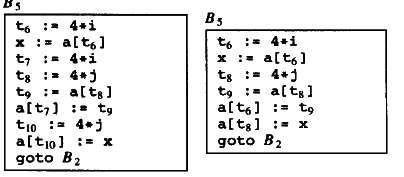
\includegraphics[scale=0.9]{Imagens/comp_1.png}
    \centering
    \caption{Antes e Depois Otimização por Subexpressão.}
    \label{subexpressao}
\end{figure}

\textbf{Propagação de Cópias:} consiste basicamente na geração de novas variáveis ou expressões para centralizar e eliminar expressões repetidas no código, conforme pode ser visualizado na figura \ref{propagacao} a seguir onde as expressões de atribuição de a e b, por serem comuns, foram centralizadas em c. 

\begin{figure}[!htb]
    \centering
    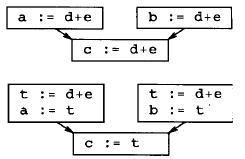
\includegraphics[scale=0.9]{Imagens/comp_2.png}
    \centering
    \caption{Propagação de Cópias.}
    \label{propagacao}
\end{figure}

\textbf{Eliminação de Código Morto:} uma variável pode ser considerada como viva em determinado ponto do programa, caso o seu valor possa ser usado subsequentemente. Caso contrário, será considerada como morta, e é nesse ponto que esta forma de transformação atua, eliminando esta variável em tempo de compilação, ou até mesmo substituindo a mesma por uma constante, o que é conhecido como transposição para constantes. Vale destacar, que um programador normalmente tende a não produzir o código morto intencionalmente, contudo durante a execução do código o mesmo pode surgir como resultado da execução e de transformações advindas da mesma.

\textbf{Otimização de Laços:} normalmente um dos principais focos de otimização, os laços, principalmente os mais internos, costumam requisitar um extenso tempo das execuções, dessa forma, é possível reduzir consideravelmente o tempo de execução de um programa ao decrementar o número de instruções de um laço mais interno, mesmo em troca de aumentar a quantidade de código fora do mesmo. Neste pontos, 3 (três) técnicas são bastante utilizadas, como a movimentação de código (toma uma expressão presente dentro do laço e que produz resultado constante e insere fora do laço, antes do mesmo), eliminação das variáveis de indução (eliminação de variáveis internas de indução, destacando que sempre uma pelo menos deve restar conforme Figura \ref{eliminacao_inducao}) e redução de carga (substituição de uma operação mais cara e complexa por outras mais barata e simples, como a troca de multiplicação por adição, conforme Figura \ref{reducao}).

\begin{figure}[!htb]
    \centering
    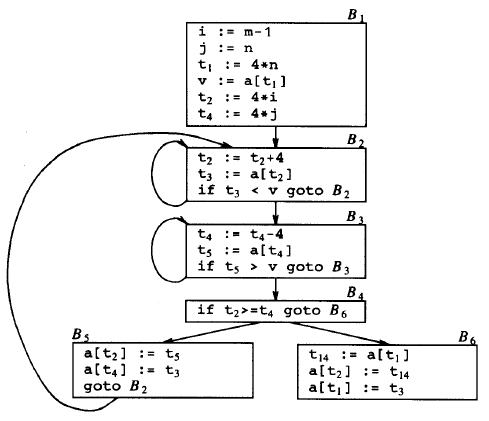
\includegraphics[scale=0.9]{Imagens/eliminacao_variavel_inducao.png}
    \centering
    \caption{Eliminação Variável de Indução.}
    \label{eliminacao_inducao}
\end{figure}

\begin{figure}[!htb]
    \centering
    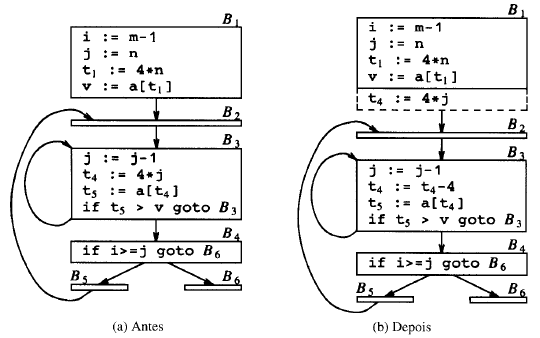
\includegraphics[scale=0.9]{Imagens/reducao_carga.png}
    \centering
    \caption{Redução de Carga.}
    \label{reducao}
\end{figure}

\bibliographystyle{sbc}
\bibliography{sbc-template}

\end{document}

